\documentclass{beamer}
\usepackage[utf8]{inputenc}
\usepackage{graphicx}
\usepackage{listings}

\usepackage{xcolor}

\lstdefinestyle{base}{
	language=C++,
	emptylines=1,
	breaklines=true,
	basicstyle=\ttfamily\color{black},
	moredelim=**[is][\bf\color{red}]{@}{@},
}

\usetheme[]{boxes}
\usecolortheme{seagull}
%\usepackage{french}
\title{Modèles et techniques en programmation parallèle hybride et multi-c\oe urs}
\subtitle{Introduction, rappels sur l'architecture matérielle, différents types de parallélismes}
\author{Marc Tajchman}\institute{CEA - DEN/DM2S/STMF/LMES}
\date{10/08/2020}
\begin{document}

\begin{frame}
\titlepage
\end{frame}

\large
\begin{frame}
\section{Rappels sur l'architecture mat\'erielle}
\frametitle{Rappels sur l'architecture mat\'erielle}

La plupart des ordinateurs actuels ont des fonctionnalités parallèles  (exécution simultanée de plusieurs traitements) : 

\begin{itemize}
	\item Les ordinateurs personnels (ordinateurs portables ou de bureau, téléphones portables, tablettes, etc.) ont presque toujours des unités de calcul (ou cœurs) multiples.
	
	Dans chaque cœur, il y a souvent plusieurs circuits arithmétiques (addition, multiplication, etc), des pipelines.
	
	\item Beaucoup d'ordinateurs ont de plus des dispositifs spécialisés dans le calcul (exemple: (GP)GPU, carte graphique utilisée pour du calcul ``massivement parallèle'')
	
	\item Les machines parallèles regroupent plusieurs nœuds de calcul (chaque noeud de calcul est similaire à un ordinateur personnel, sans clavier, ni souris), les nœuds de calculs sont connectés entre eux.
\end{itemize}
\end{frame}

\begin{frame}

\textcolor{red}{Machine parallèle typique}: 
\begin{itemize}
	\item un ensemble de n\oe uds de calcul chacun contenant un ou plusieurs cœurs et de la m\'emoire, parfois un GPU
	\item les nœuds sont connect\'es entre eux par un r\'eseau
	\item et aussi à un système qui gère les données d'entrée et produites (disques partagés)
	\item les utilisateurs ne se connectent pas directement aux noeuds de calcul mais passent par un frontal (ordinateur qui gère les connexions multiples à la machine parallèle)
\end{itemize}

\vfill
\begin{center}
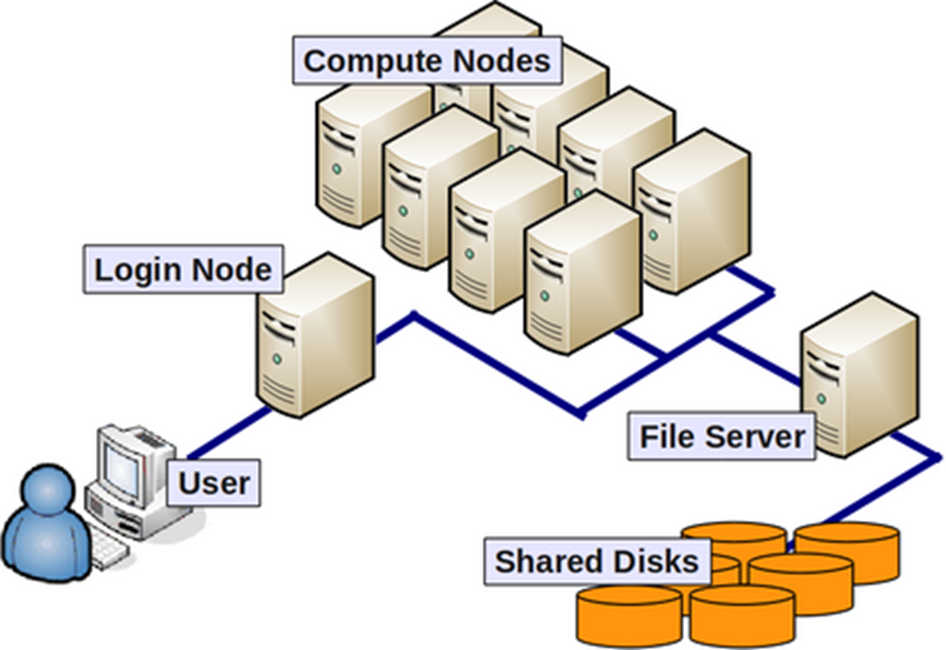
\includegraphics[scale=0.14]{../../Images/ParallelMachine.png}
\end{center}

(les machines les plus puissantes actuellement contiennent plusieurs centaines de milliers de n\oe uds)
\end{frame}

\begin{frame}
Schéma interne d'un n\oe ud (variable suivant le mod\`ele de processeur et la g\'en\'eration utilis\'ee):

\begin{center}
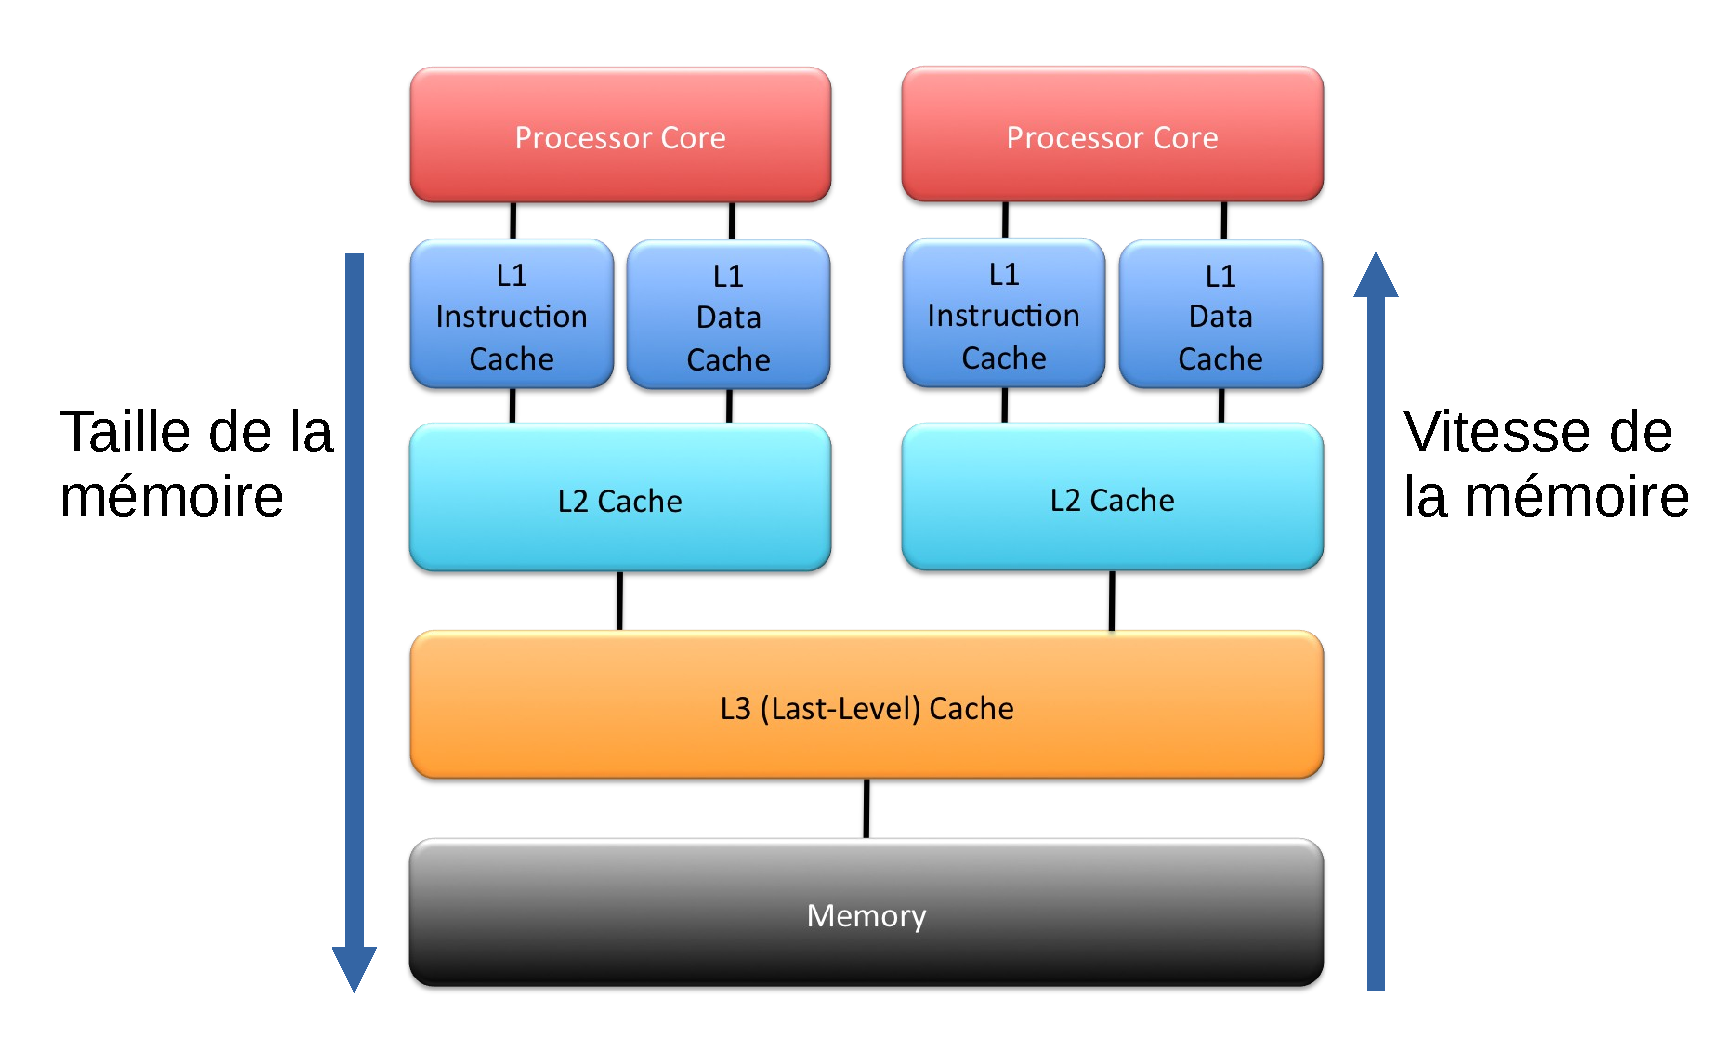
\includegraphics[scale=0.32]{../../Images/NoeudCalcul}
\end{center}

\end{frame}

\begin{frame}

Exemple : processeur AMD Ryzen 4900
\begin{center}
	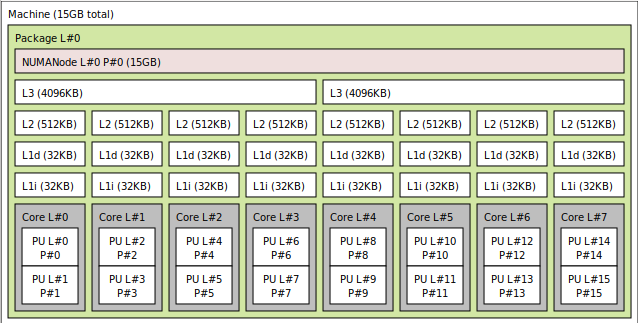
\includegraphics[scale=0.32]{../../Images/lstopo_ryzen_4900}
\end{center}

Exemples : processeurs Intel i5 8400H - i9 9900K
\begin{center}
	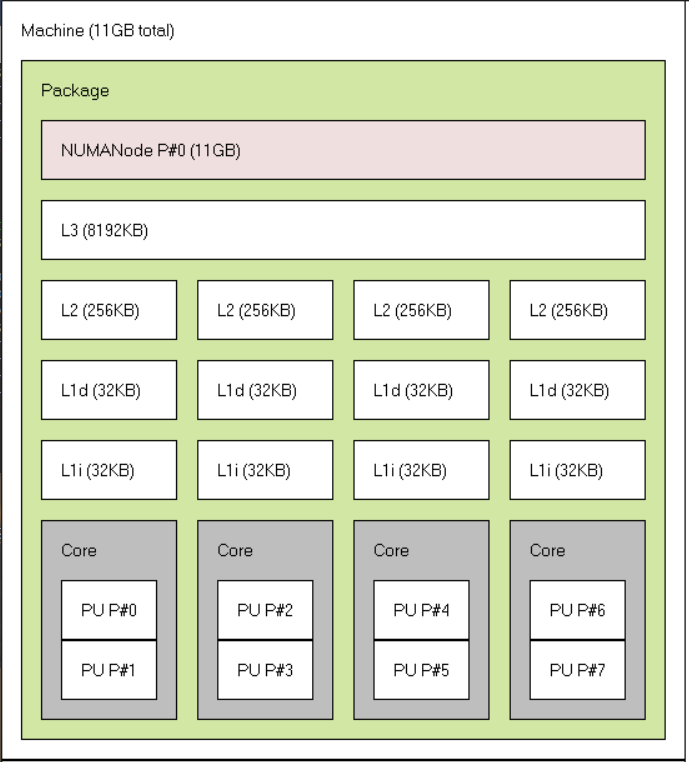
\includegraphics[scale=0.23]{../../Images/topo_i5}
	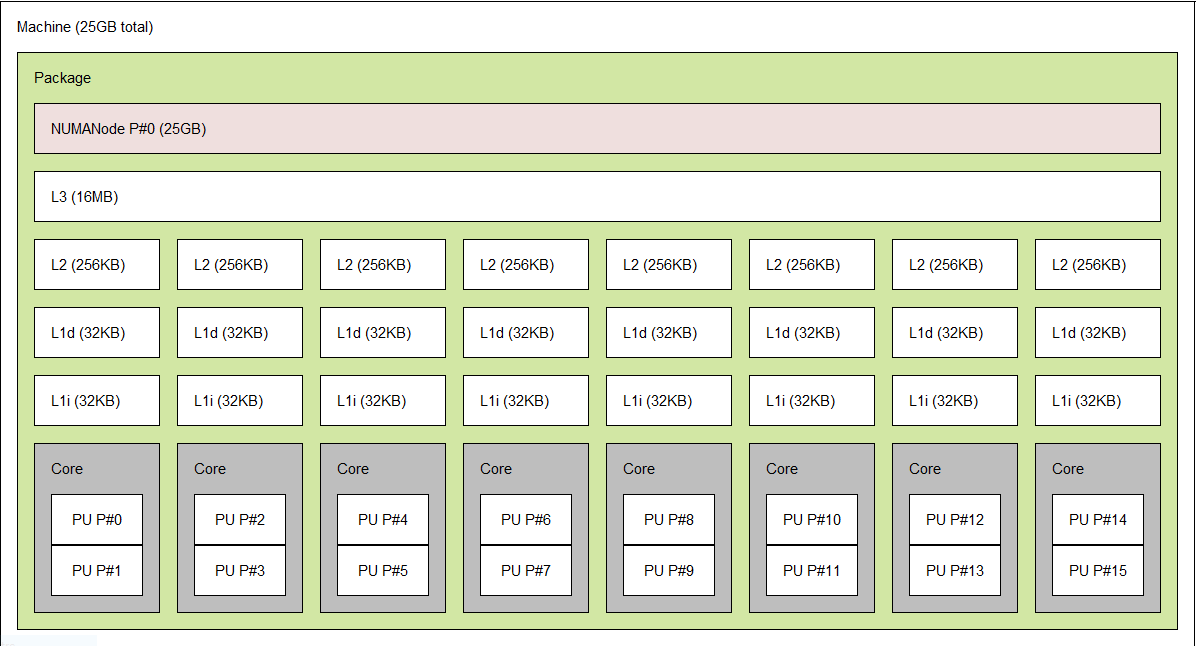
\includegraphics[scale=0.23]{../../Images/topo_i9}
\end{center}

\end{frame}

\begin{frame}[fragile]
Jusque 6 types de mémoires différentes:
\begin{itemize}
\item registres : mémoire très rapide dans chaque cœur
\item mémoires caches L1, L2, L3 : mémoires rapides, partagées partagées entre une partie des cœurs
\item mémoire centrale : mémoire moins rapide mais de plus grande taille
\item disques : mémoire lente.
\end{itemize}

A noter que la différence entre mémoire centrale et disque tend à diminuer avec la généralisation des SSD.

\bigskip
\begin{center}
	\framebox{%
	\begin{minipage}{9cm}
	\textcolor{red}{Les échanges entre la mémoire centrale et les mémoires cache se font par blocs de données (appelées ``lignes de cache'') et pas ``à l'unité'' pour des raisons de performances.}
    \end{minipage}
    }
\end{center}

\end{frame}

\begin{frame}
Schéma interne d'un c\oe ur (variable suivant le mod\`ele de processeur et la g\'en\'eration utilis\'ee):

\begin{center}
	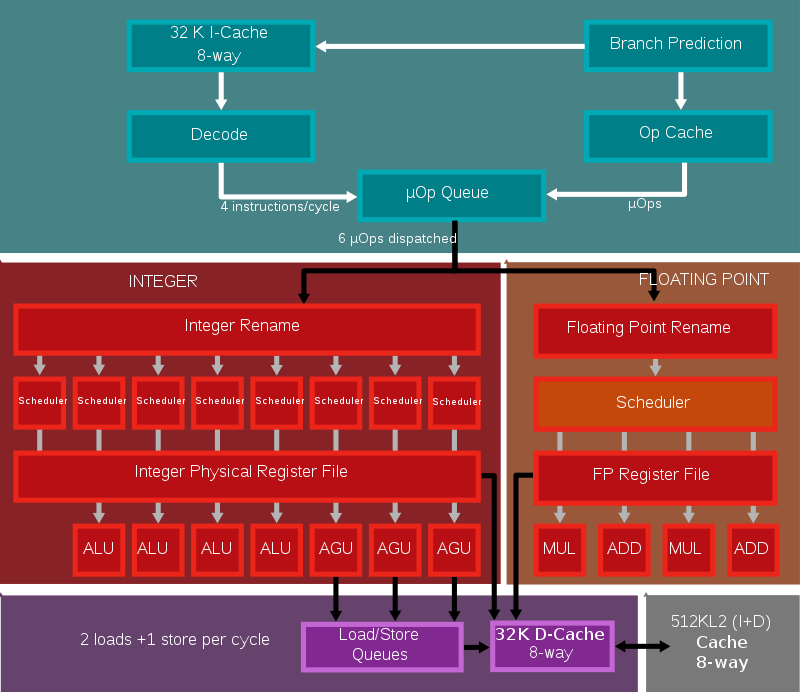
\includegraphics[scale=0.25]{../../Images/800px-Zen2_Microarchitektur.svg.png}
	
	AMD - Zen2 $\mu$arch (simplifi\'e)
\end{center}

\end{frame}

\begin{frame}[fragile]
Situation actuelle (et encore pour plusieurs ann\'ees): 
\begin{quote}
	
	\vfill
	vitesse de calcul (d'un processeur)
	\vfill
	
	\begin{itemize}
		\item[$\approx$] vitesse de la m\'emoire interne (registres) du processeur
			\medskip
	        
		\item[$>$] vitesse des diff\'erentes m\'emoires cache, interm\'ediaires entre le processeur et la m\'emoire centrale du n\oe ud
		
		\hfill (vitesse L1 $>$ L2 $>$ L3, 
		
		\hfill taille L1 $<$ L2 $<$ L3)
			\medskip
			
		\item[$\gg$] vitesse de la m\'emoire centrale d'un n\oe ud
			\medskip
			
		\item[$\gg$] vitesse du r\'eseau qui connecte les n\oe uds
	\end{itemize}


\end{quote}

\end{frame}

\begin{frame}

La gestion des différentes mémoires est faite par une puce appelée contrôleur mémoire.
\bigskip

Fonctionnement :

\begin{itemize}
	\item Quand un c\oe ur  a besoin d'une donn\'ee, il la demande au contrôleur m\'emoire.
	\vfill
	
	\item Le gestionnaire m\'emoire regarde si la donn\'ee est dans la m\'emoire cache L1, L2 ou L3 de ce processeur, sinon le bloc de la m\'emoire centrale qui contient la donn\'ee est recopi\'e dans la m\'emoire cache (dans L3, puis L2 et  L1).
	
	\vfill
	\item Ensuite, la donn\'ee est recopi\'ee dans un registre de ce c\oe ur.
	
	\vfill
\end{itemize}
\end{frame}

\begin{frame}

\vfill
\begin{itemize}
\item Quand un c\oe ur a modifi\'e une donn\'ee, il le notifie au gestionnaire m\'emoire
\vfill
\item Le gestionnaire m\'emoire recopie la donn\'ee vers la m\'emoire cache (L1, L2 puis L3) et vers la m\'emoire centrale
\vfill
\item Il v\'erifie aussi qu'une autre copie de la donn\'ee n'existe pas dans la m\'emoire cache d'un autre c\oe ur.
\vfill
\item Si c'est le cas, les autres copies sont mises \`a jour
\end{itemize}
	\vfill
\end{frame}

\begin{frame}[fragile]
	
	\vfill
Ce système s'est généralisé parce qu'il est très compliqué/cher de produire de la mémoire qui suive les performances des processeurs. 

Permet de maintenir de bonnes performances avec de la mémoire de grande taille mais plus lente.
	\vfill
{\bf Cette gestion peut repr\'esenter une partie im\-por\-tante du temps d'ex\'ecution de programmes parallèles (pour assurer la coh\'erence des diff\'erentes parties de la m\'emoire et leurs mises \`a jour correctes).}
	\vfill	
	
\end{frame}
\begin{frame}
	Ce qu'il faut retenir:

	\begin{itemize}
		\item \textcolor{blue}{En général, plusieurs niveaux de parallélisme disponibles}
		\begin{enumerate}
			\item Entre les nœuds de calcul (avec par ex. MPI)
			\item Entre les cœurs dans un même nœud de calcul (avec par ex. MPI ou OpenMP)
			\item Dans un cœur, entre les circuits arithmétiques 
			\item Dans un GPU (avec par ex. Cuda/OpenCL)
		\end{enumerate}
		\medskip
		
		\item  \textcolor{blue}{On peut combiner ces différents niveaux de //} (en faisant un peu attention) 
		\medskip
		
		\item  \textcolor{blue}{Dans ce cours, on s'intéressera principalement:}
		\begin{itemize}
			\item au // entre cœurs (OpenMP)
			\item au // dans un GPU
			\item au // mixte (MPI/OpenMP/Cuda)
		\end{itemize}
		\medskip
		\item \textcolor{blue}{Tous les ordinateurs actuels utilisent de la mémoire cache}
	
	    La mémoire cache est là pour améliorer la différence entre la vitesse des processeurs et la vitesse d'accès à la mémoire centrale.
	\end{itemize}
\end{frame}



\end{document}
